%!TEX root = ../intro.tex
%******************************
%	 Bayesian approaches
%*****************************

\section{Bayesian approaches to model scRNA-Seq data}

In the last decade, an array of tools to process and analyse scRNA-Seq data has been developed. These methods include tools for data acquisition (e.g.~alignment, de-duplication, quantification), data filtering (e.g.~quality control, normalisation, imputation), cell labelling (e.g.~clustering, classification, ordering) and gene-level analysis (e.g.~differential expression, detection of expression patterns) \citep{Zappia2018}. Extensive comparisons of these methods have been performed for each stage of the analysis pipeline \citep{Saelens2018, Soneson2018}. In this thesis, I will focus on the application and development of Bayesian statistical methodologies designed to characterise cellular heterogeneity using scRNA-Seq data. This section describes key concepts of Bayesian inference and related previous work that serve as a foundation for the results in later chapters.

\subsection{The basics of Bayesian inference}

The main difference between classical and Bayesian inference is the treatment of model parameters. While classical inference considers model parameters as fixed but unknown values, Bayesian approaches treat parameters as random variables for which probability distributions quantify uncertainty \citep{Bernardo2003}. In this context, prior beliefs about the distribution of the model parameter $\omega$ are summarised in the form of a \emph{prior distribution} $\pi(\omega)$. Once the data $D$ is observed, the prior distribution is updated using the Bayes theorem \cite{Bayes1763} to form the posterior distribution $\pi^*(\omega|D)$:

\begin{equation} \label{eq0:Bayes_theorem}
\pi^*(\omega|D)=\frac{L(D|\omega)\pi(\omega)}{L(D)}\text{, where }L(D)=\int_\omega{}L(D|\omega)\pi(\omega)d\omega 
\end{equation}

Here, $L(D|\omega)$ is the likelihood of observing the data given the parameter $\omega$ and $L(D)$ is the marginal likelihood after integrating out the parameter $\omega$. As discussed in \textbf{Section \ref{sec0:prior}}, $L(D)$ does not have a closed form, except for specific prior choices. Despite this, the numerical methods described in \textbf{Section \ref{sec0:posterior_inference}} enable estimating the posterior distribution $\pi^*(\omega|D)$ without the need of calculating $L(D)$.

\newpage

\subsection{Prior distributions}
\label{sec0:prior}

The role of the prior distribution is to incorporate prior knowledge about the model parameters. Using the Bayes theorem, this is then combined with the data to form the posterior distribution. For this purpose, a prior distribution should ideally describe the experimenter's prior knowledge regarding the unknown parameters (e.g.~based on previous experiments). For practical use, the prior distribution can be chosen to form an analytically tractable solution for the integral that is required to calculate $L(D)$. This is achieved by using conjugate prior distributions, for which the prior is of the same family as the posterior distribution. As such, conjugate prior distributions lead to a closed form posterior distribution, which facilitates posterior inference. A list of commonly used conjugate prior distributions can be seen in \textbf{Table \ref{tab0:priors}} which was taken from Fink \emph{et al.}, 1997 \citep{Fink1997}.

\begin{table}[hb	]
\centering
\caption[Conjugate prior distributions for common likelihood functions]{Conjugate prior distributions for common likelihood functions.}
\label{tab0:priors}
\begin{tabular}{l l l}
\toprule
\textbf{Discrete} & &\\
\midrule
\midrule
\textbf{Data generation process} & \textbf{Prior} & \textbf{Posterior} \\ 
\midrule 
Bernoulli & Beta & Beta \\
Poisson & Gamma  & Gamma \\
Negative Binomial & Beta & Beta \\
\midrule
\midrule
\textbf{Continuous} & & \\
\midrule
\midrule
\textbf{Data generation process} & \textbf{Prior} & \textbf{Posterior} \\ 
\midrule
Uniform  & Pareto & Pareto \\ 
Normal (unknown mean) &  Normal  & Normal \\ 
Normal (unknown variance) &  Inverse Gamma  & Inverse Gamma \\ 
Gamma (unknown rate) &  Gamma  & Gamma \\ 
Exponential &  Gamma  & Gamma \\ 
\bottomrule
\end{tabular}
\end{table} 

When prior knowledge of the model parameters is not available, non-informative or objective priors may be used (e.g.~the Jeffreys prior \citep{Jeffreys1946}). However, a detailed discussion regarding such priors is outside the scope of this thesis.

\subsection{Posterior inference} \label{sec0:posterior_inference}

Before the wide availability of computers, Bayesian research centred around finding pairs of likelihood functions and prior distributions that produce well-defined and tractable solutions for posterior distributions (conjugate priors). More recently, the increase in computing power supported the development of numerical methods to approximate the integrals needed to form posterior distributions \citep{Fink1997}. Numerical approximations are frequently needed when objective priors are used or for models with large complexity. Here, I will focus on \gls{MCMC} \citep{Metropolis1953, Hastings1970}, one of the most popular strategies to approximate posterior distributions. The idea behind MCMC is to generate a random sample of the posterior distribution $\pi^*(\omega|D)$ when this distribution cannot be obtained in closed form. For this, a Markov chain is simulated over $n$ iterations whose equilibrium distribution is $\pi^*(\omega|D)$ \citep{Bernardo2000}. Extensive research led to the development of algorithms that generate this equilibrium distribution \citep{Casella1992, Gelfand1990, Greyer1992, Besag1993, Gelman1992}. The following two examples of MCMC are commonly used for a range of applications in Bayesian statistics \citep{Bernardo2000}.

\subsubsection{Gibbs sampling}

Consider a statistical model for which $\bm{\theta}=(\theta_1,...,\theta_K)$ represents a vector of unknown parameters. If the joint posterior $\pi^*(\bm{\theta}|D)=\pi^*(\theta_1,...,\theta_K|D)$ is not tractable, it may be numerically approximated. For each model parameter $\theta_k$, one defines the \emph{full conditional} distribution as:

\begin{equation}
\pi^*(\theta_k|D,\theta_{k'},k'\neq{}k), \quad k=1,...,K
\end{equation}

This is the density of the individual component $\theta_k$, given the data and specified values of all other components $\theta_{k'}$ \cite{Geman1984} For each iteration $t$ with $t=1,...,T$:

\begin{align*}
\textnormal{draw} \quad  \theta_1^{(t+1)} \quad \textnormal{from} \quad & \pi^*(\theta|D, \theta_2^{(t)},...\theta_K^{(t)})\\
\textnormal{draw} \quad  \theta_2^{(t+1)} \quad \textnormal{from} \quad & \pi^*(\theta|D, \theta_1^{(t+1)},\theta_3^{(t)},...\theta_K^{(t)})\\
&.\\
&.\\
&.\\
\textnormal{draw} \quad  \theta_K^{(t+1)} \quad \textnormal{from}  \quad& \pi^*(\theta|D, \theta_1^{(t+1)},...\theta_{K-1}^{(t+1)})
\end{align*}

For $t\rightarrow{}\infty$ the joint distribution of $(\theta_1^{(t)},...,\theta_k^{(t)})$ converge to the posterior distribution $\pi^*(\bm{\theta}|D)$ \citep{Roberts1994, Geman1984}. The implementation of Gibbs sampling is straightforward when the full conditionals have a known form. Alternatively, stochastic simulation techniques can be used to generate draws from one or more full conditionals.

\subsubsection{Metropolis-Hastings}

One of these techniques is the \emph{Metropolis-Hastings algorithm} \citep{Metropolis1953, Hastings1970} which constructs a Markov chain $\theta_k^{(1)},...,\theta_k^{(T)}$ as follows:\\
For each iteration $t=1,...,T$, let $q(\theta_k^{(t)},\theta_k')$ be a proposal distribution for which, given a current draw $\theta_k^{(t)}$, a candidate value $\theta_k'$ is proposed. Subsequently, with some probability $\alpha(\theta_k^{(t)},\theta_k'|\theta_{k'}^{(t)},k'\neq{}k)$ the proposed value $\theta_k'$ is accepted (i.e.~$\theta_k^{(t+1)}=\theta_k'$) and otherwise rejected ($\theta_k^{(t+1)}=\theta_k^{(t)}$) \cite{Roberts1994, Hastings1970}. In practice, the update is performed as follows:

\begin{enumerate}
\item Sample $\nu\sim\textnormal{Unif(0,1)}$ and a candidate $\theta_k'$ from $q(\theta_k^{(t)},\theta_k')$.
\item Define

\begin{equation}
\alpha(\theta_k^{(t)},\theta_k'|\theta_{k'}^{(t)},k'\neq{}k)=\min\left\lbrace{}1,\frac{\pi^*(\theta_k'|D,\theta_{k'}^{(t)},k'\neq{}k)q(\theta_k',\theta_k^{(t)})}{\pi^*(\theta_k^{(t)}|D,\theta_{k'}^{(t)},k'\neq{}k)q(\theta_k^{(t)},\theta_k')}\right\rbrace
\end{equation}

\item If $\nu\leq{}\alpha(\theta_k^{(t)},\theta_k'|\theta_{k'}^{(t)},k'\neq{}k)$, set $\theta_k^{(t+1)}=\theta_k'$ otherwise set $\theta_k^{(t+1)}=\theta_k^{(t)}$
\end{enumerate}

For this algorithm, the proposal distribution $q(\theta_k^{(t)},\theta_k')$ needs to be chosen. A common choice is a Normal distribution centred at $\theta_k^{(t)}$, where the variance needs to be selected to have some level of optimality in the performance of the algorithm \citep{Roberts2001}. An automated tuning process for the variance of the proposal distribution $q(\theta_k^{(t)},\theta_k')$ was introduced by Roberts and Rosenthal, 2009 \citep{Roberts2009}. This \emph{adaptive Metropolis-Hastings} algorithm is often used in combination with Gibbs sampling (\emph{adaptive Metropolis-within-Gibbs sampling}) to approximate the posterior distribution of model parameters for complex models \citep{Roberts2009}.

\subsubsection{Practical considerations}

When an MCMC sampler is chosen, one needs to assess the convergence of the chain. For this purpose, the initial iterations of the MCMC algorithm are typically discarded (\emph{burn-in}). Within the burn-in period, the autocorrelation of the chain is expected to decay to a negligible level \citep{Greyer1992}. After burn-in, one can compute the autocorrelation of the chain to assess how well the chain mixed. High autocorrelation suggest that subsequent MCMC draws are similar, and therefore the chain explores the parameter space slowly (i.e.~it may take a long time before the chain converges). The standard deviation of the chain (as a measure of statistical uncertainty) is defined as:

\begin{equation}
\sigma=\frac{\sigma^*}{\sqrt{T}}\sqrt{\frac{1+\rho}{1-\rho}}
\end{equation}

Here, $\sigma^*$ is the posterior standard deviation of $\pi^*(\omega|D)$, $T$ is the sample size and $\rho$ the autocorrelation \citep{Tierney1991}. Therefore, $\sigma$ decreases when $\rho$ is small. This also supports finding an optimal run length until sufficient mixing is achieved. In practice, storing only every 10 or 100 samples (thinning) reduces autocorrelation of the chain and reduces storage requirements \citep{Greyer1992}. One formal way of assessing the convergence of the chain was introduced by Geweke, 1992. Here, the means of the first 10\% and the last 50\% of the samples are compared. If the means are different, this test suggests that the chain has not yet reached equilibrium \citep{Geweke1992}. Alternatively, graphical summaries, such as traceplots, can be used to formally assess convergence.

\subsection{Variational Bayes}

When datasets are large and models are complex, the above described MCMC sampling methods are slow to derive posterior distributions. Instead, variational inference can derive an approximate posterior distribution using optimisation, rather than sampling. The principle of variational inference is to select a member of a family of densities $Q$ by minimising the \gls{KL}:

\begin{equation}
q^\ast(\bm{\theta})=\underset{q(\bm{\theta})\in{}Q}{\textnormal{argmin\,{}KL}}(q(\bm{\theta})||\pi^*(\bm{\theta}|D))
\end{equation}

A common choice in variational Bayesian approaches is to assume that model parameters are mutually independent so that the \emph{mean-field variational family} of distributions can be chosen for $q(\bm{\theta})$:

\begin{equation}
q(\bm{\theta})=\prod_{j=1}^k{}q_j(\theta_j)
\end{equation}

Here, each model parameter $\theta_j$ is governed by its own variational factor \citep{Blei2017}.\\

The posterior distribution is then approximated by $q^\ast(\bm{\theta})$\citep{Blei2017}. In general, variational inference tends to be faster than MCMC, albeit MCMC allows producing exact samples from the target density \citep{Blei2017}. Therefore, variational inferences may be preferred when datasets are large and exact samples are not needed. A common approach to minimise the KL is to maximise the \gls{ELBO} (see e.g.~\citep{Beal2003}) which is defined as:

\begin{equation}
\textnormal{ELBO}(q)=\mathbb{E}[\log(L(D|\bm{\theta})\pi(\bm{\theta}))] - \mathbb{E}[\log(q(\bm{\theta}))]
\end{equation}

One commonly used technique to maximise the ELBO is \emph{\gls{CAVI}}. Similar to Gibbs sampling, CAVI maximises the ELBO for one parameter while keeping all other parameters constant. This is done iteratively until the ELBO converges against a local maximum \citep{Blei2017}. 

\subsection{Bayesian decision theory} \label{sec0:decision}

Assume the data $D$ have arisen under one of the models $M_1$ or $M_0$. The posterior probabilities for each model are denoted as $\pi^*(M_1|D)$ and $\pi^*(M_0|D)$. Similarly, prior probabilities for each model are denoted as $\pi(M_1)$ and $\pi(M_0)$. The Bayes factor $B_{10}$ \citep{Jeffreys1961} is defined as the ratio of the posterior odds of $M_1$ to its prior odds:

\begin{equation}
B_{10}=\frac{\pi^*(M_1|D)}{\pi^*(M_0|D)}/{}\frac{\pi(M_1)}{\pi(M_0)}=\frac{L(D|M_1)}{L(D|M_0)}
\end{equation}  

When the models $M_1$ and $M_0$ are equally probable \emph{a priori}, the Bayes factor is equal to the posterior odds in favour of $M_1$ \citep{Kass1995}. To compute the Bayes factor, one needs to find the marginal likelihoods $L(D|M_1)$ and $L(D|M_0)$ (see equation \eqref{eq0:Bayes_theorem}). Typically, these marginal likelihoods are intractable and this measure is difficult to compute. \\

Alternatively, \emph{tail posterior probabilities} can be computed as a selection rule regarding $M_1$ and $M_0$ when these models are defined by restrictions in the parameter space (e.g.~$M_1:\theta\in\Theta$ versus $M_0:\theta\notin\Theta$). For example, posterior tail probabilities were introduced to test the difference $\delta_g$ in log-expression of gene $i$ between condition $A$ and condition $B$ \citep{Bochkina2007}. Here, the posterior tail probability of $\delta_g$ being larger than a given threshold $\delta_g^{(\alpha)}$ is defined as:

\begin{equation}
\pi(\delta_g,\delta_g^{(\alpha)})=P\left\lbrace|\delta_g|>\delta_g^{(\alpha)}|D\right\rbrace
\end{equation}

In the case of testing changes in mean expression, the difference $\delta_g$ represents the log-fold change in mean expression ($\log(\frac{\mu^{(B)}}{\mu^{(A)}})$). In practice, for each iteration of the MCMC, this difference is computed and the tail posterior probability is the fraction of the absolute distance being larger than the threshold. If the tail posterior probability is larger than an evidence threshold (e.g. 80\%) one would reject the null hypothesis $|\delta_g|\leq\delta_g^{(\alpha)}$ \citep{Vallejos2016}. 

\subsection{Modelling scRNA-Seq data}

Several approaches have been proposed to estimate model parameters based on scRNA-Seq data. Commonly, the count data is modelled as \gls{NB} distributed \citep{Vallejos2015BASiCS, Risso2018, Lopez2018}. The NB distribution is defined as:

\begin{equation}
f_{NB}(y;\mu,\theta)=\frac{\Gamma(y+\theta)}{\Gamma(\theta)y!}\left(\frac{\theta}{\theta + \mu}\right)^\theta\left(\frac{\mu}{\mu + \theta}\right)^y
\end{equation}

Here, the dispersion of the NB is $\delta=\theta^{-1}$ \cite{Risso2018}. In terms of a hierarchical model, the NB can be decomposed as a Poisson distribution with a Gamma random effect \cite{Vallejos2015BASiCS}:

\begin{align*}
y|\cdot&\sim{}\textnormal{Poisson}(\nu\mu)\\
\nu|\alpha,\beta&\sim{}\textnormal{Gamma}(\alpha,\beta)
\end{align*}

In some cases \citep{Risso2018, Lopez2018} the NB is extended to account for dropout events in scRNA-Seq data \citep{Kharchenko2015}. The \gls{ZINB} takes the form:

\begin{equation}
f_{ZINB}(y;\mu,\theta,\pi)=\pi\delta_0(y) + (1-\pi)f_{NB}(y;\mu,\theta) 
\end{equation}

where $\delta_0(\cdot)$ is the Dirac function and $\pi\in[0,1]$ is the probability that 0 is observed instead of the count $y$ \citep{Risso2018}. Nevertheless, it has been shown that the zero inflation is not needed to capture expression dropouts as it can be modelled by the over-dispersion in the NB distribution \citep{Lopez2018}. In a hierarchical formulation this model writes as:

\begin{align*}
y|\cdot & = 
 \left\lbrace
  \begin{aligned}
    & x && \textnormal{if} \; h = 0,  \\ 
    & 0 && \textnormal{otherwise}    	    
  \end{aligned}
\right.\\
x|\cdot&\sim{}\textnormal{Poisson}(\nu\mu)\\
h & \sim \textnormal{Bernoulli}(\cdot)\\
\nu|\alpha,\beta&\sim{}\textnormal{Gamma}(\alpha,\beta)
\end{align*}

Other approaches model scRNA-Seq counts as log-normally distributed \citep{Azizi2017,Pierson2015}. \Gls{ZIFA} assumes that the data $Y=[y_1,...,y_N]$, where $N$ is the number of samples with $D$ genes, are generated from an unobserved low-dimensional space $Z=[z_1,...,z_N]$ with dimension $K,\,{}K\ll{}D$ \citep{Pierson2015}. The generation process is a linear transformation with added Gaussian noise from the latent space ($N\times{}K$) into the latent high-dimensional gene expression space with dimension $N\times{}D$. Additionally, with some probability being a function of the latent expression level of gene $j$ in cell $i$ $x_{ij}$: $p_0=\exp(-\lambda{}x_{ij}^2)$, a dropout is observed \citep{Pierson2015}. The full model is defined as:

\begin{align*}
y_{ij} & = 
 \left\lbrace
  \begin{aligned}
    & x_{ij} && \textnormal{if} \; h_{ij} = 0,  \\ 
    & 0 && \textnormal{otherwise}    	    
  \end{aligned}
\right.\\
\bm{x}_{i}|\bm{z}_i&\sim{}\textnormal{Normal}(\bm{Az}_i+\bm{\mu},\bm{W})\\
h_{ij}|x_{ij} & \sim \textnormal{Bernoulli}(p_0)\\
\bm{z_i}&\sim{}\textnormal{Normal}(0,\bm{I})
\end{align*} 

Here, $\bm{A}$ denotes a $D\times{}K$ factor loadings matrix, $\bm{\mu}$ a $D\times{}1$ mean vector, $\bm{W}$ a $D\times{}D$ covariance matrix and $\bm{I}$ the $K\times{}K$ identity matrix.

\subsection{BASiCS: Bayesian Inference of Single-Cell Sequencing data} 
\label{sec0:BASiCS}

Throughout this thesis, I will use and extend the \gls{BASiCS} framework \citep{Vallejos2015BASiCS, Vallejos2016}. BASiCS models scRNA-Seq data generated from seemingly homogeneous populations of cells (i.e.~where no distinct sub-populations are found) to perform down-stream analysis (e.g. normalisation, differential expression testing).\\

In BASiCS, the expression count of gene $i$ ($ \in \{1, \ldots, q\}$) in cell $j$ ($\in \{ 1, \ldots ,n\}$) $X_{ij}$ is treated as a random variable. Compared to bulk RNA-Seq, scRNA-Seq is inherently noisy due to low starting amounts of RNA \citep{Brennecke2013}. To control for technical noise, BASiCS incorporates reads from synthetic RNA spike-ins \citep{Jiang2011}. Here, the first $q_0$ genes are biological and the  remaining $q-q_0$ genes are technical.

\begin{equation} 
 X_{ij}|\mu_i,\phi_j,\nu_j,\rho_{ij} \sim
 \left\lbrace
  \begin{aligned}
    &\textnormal{Poisson}(\phi_j\nu_j\mu_i\rho_{ij}), && i=1,...,q_0,j=1,...n;  \\ 
    &\textnormal{Poisson}(\nu_j\mu_i), && i=q_0+1,...,q,j=1,...,n,    	    
  \end{aligned}
\right.
\end{equation} 

In this model, two random effects were added to model the technical and biological part of the over-dispersion:

\begin{equation} 
\nu_j|s_j,\theta \sim \textnormal{Gamma}\left(\frac{1}{\theta},\frac{1}{s_j\theta}\right), \hspace{0.2cm} \rho_{ij}|\delta_i  \sim \textnormal{Gamma}\left(\frac{1}{\delta_i},\frac{1}{\delta_i}\right)\\
\end{equation} 

Note that this formulation relates to the hierarchical representation of the NB distribution, but this model is more general as two sets of random effects are incorporated. Here, $\phi_j$ represents a cell-specific normalisation parameter to correct for differences in mRNA content between cells and $s_j$ models cell-specific scale differences affecting all biological and technical genes (e.g.~amplification biases or RNA capture biases). Moreover, the random effect $\nu_j$ captures unexplained technical noise that is not accounted for by the normalisation. The strength of this noise is then quantified by a global parameter $\theta$ (shared across all genes and cells). Heterogeneous gene expression across cells is captured by $\rho_{ij}$, whose strength is controlled by gene-specific over-dispersion parameters $\delta_i$. These quantify the excess of variability that is observed with respect to Poisson sampling noise, after accounting for technical noise. Finally, gene-specific parameters $\mu_i$ represent average expression of a gene across cells \textbf{(Fig.~\ref{fig0:BASiCS}A)}. 

\begin{figure}[!h]
\centering
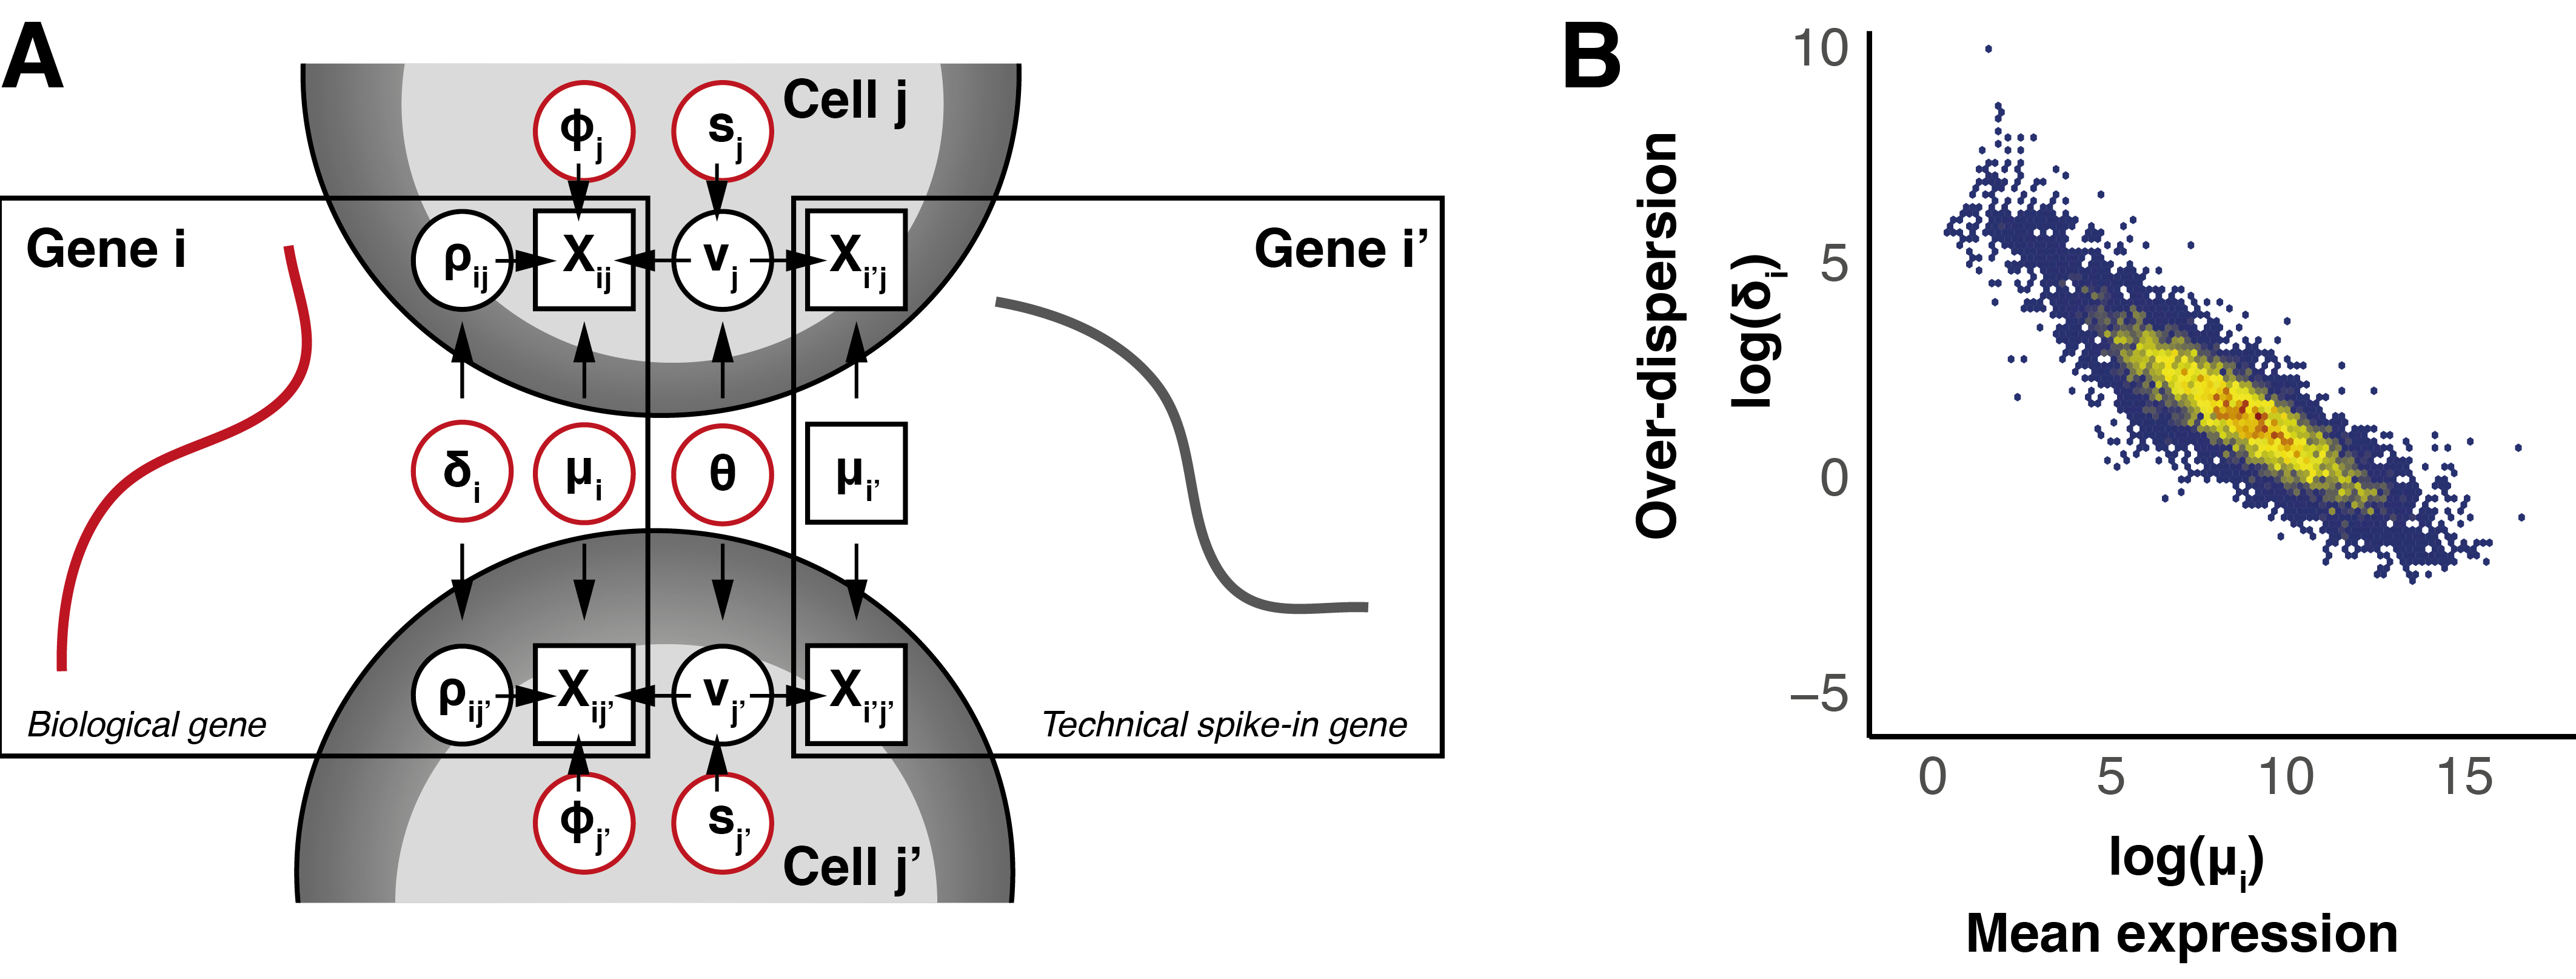
\includegraphics[width=\textwidth]{Fig_19.png}
\caption[The BASiCS model]{\textbf{The BASiCS model.}\\
\textbf{(A)} Hierarchical formulation of the statistical model underlying BASiCS visualised for two cells (j and j') and two genes (i and i', gene i' represents a technical spike-in gene). Squared nodes indicate known quantities (observed expression counts and added number of spike-in molecules). Round nodes indicate unknown quantities. Red circles represent unknown model-parameters while black circles indicate the random effects that play intermediate roles effecting expression counts. Adapted from \citep{Vallejos2015BASiCS}, \textbf{(B)} Illustration of the typical confounding effect that is observed between gene-specific estimates of over-dispersion parameters $\delta_i$ and mean expression parameters $\mu_i$.}
\label{fig0:BASiCS}
\end{figure}

Prior specifications for the model parameters are chosen as follows:

\begin{align*}
\mu_i&\sim\textnormal{log-N}(0,a_\mu^2) \quad \textnormal{for}\;{}i=1,...,q_0\\
\delta_i&\sim\textnormal{log-N}(0,a_\delta^2) \quad \textnormal{for}\;{}i=1,...,q_0\\
s_j&\sim\textnormal{Gamma}(a_s,b_s), \quad j=1,...,n\\
\theta&\sim\textnormal{Gamma}(a_\theta,b_\theta)\\
\Phi&\sim{}n\textnormal{Dirichlet}(a_\Phi), \quad \Phi=(\phi_1,...,\phi_n)
\end{align*}

\newpage

After integrating out the $\rho_{ij}$ to enhance mixing of the MCMC algorithm that was adopted to perform posterior inference \citep{Vallejos2015BASiCS} the likelihood is defined as:

\begin{align} 
\Lagr = & \left[\prod_{i=1}^{q_0}\prod_{j=1}^n\frac{\Gamma(x_{ij}+\frac{1}{\delta_i})}{\Gamma(\frac{1}{\delta_i})x_{ij}!}\left(\frac{\frac{1}{\delta_i}}{\phi_j\nu_j\mu_i+\frac{1}{\delta_i}}\right)^\frac{1}{\delta_i}\left(\frac{\phi_j\nu_j\mu_i}{\phi_j\nu_j\mu_i+\frac{1}{\delta_i}}\right)^{x_{ij}}\right] \nonumber\\ 
&\times\left[\prod_{i=q_0+1}^{q}\prod_{j=1}^n\frac{(\nu_j\mu_i)^{x_{ij}}}{x_{ij}!}\exp\lbrace-\nu_j\mu_i\rbrace\right]
\end{align} 

Given the NB model, the expected biological counts take the form:

\begin{equation}
\mathbb{E}(X_{ij}|\mu_i,\delta_i,\phi_j,s_j,\theta)=\phi_js_j\mu_i
\end{equation}

This formulation can be used to obtain normalised counts. Furthermore, the coefficient of variation is defined as:

\begin{equation}
\textnormal{CV}^2(X_{ij}|\mu_i,\delta_i,\phi_j,s_j,\theta)=\frac{1}{\phi_js_j\mu_i} + \theta + \delta_i(\theta + 1)
\end{equation}

As discussed in Vallejos \emph{et al.}, 2016 \citep{Vallejos2016}, the CV$^2$ is inversely proportional to the mean expression $\mu_i$. Furthermore, $\delta_i$ can be interpreted as the residual CV$^2$ after removing Poisson sampling and residual technical over-dispersion \citep{Vallejos2015BASiCS, Vallejos2016}. We will therefore use $\delta_i$ as a proxy for the biological part of transcriptional variability when modelling scRNA-Seq data.\\

Posterior inference is implemented using adaptive Metropolis-within-Gibbs sampling (see \textbf{Section \ref{sec0:posterior_inference}}) \citep{Vallejos2015BASiCS, Vallejos2016}. Once posterior distributions are obtained, down-stream analyses can be performed. These include: normalisation of expression counts, variance decomposition into biological and technical noise, detection of highly and lowly variable genes and differential mean and differential over-dispersion testing. The latter is done by computing the tail posterior probabilities of the difference in mean expression or over-dispersion between two conditions ($p$ and $p'$) being larger than an evidence threshold $\tau_0$ or $\omega_0$ (see \textbf{Section \ref{sec0:decision}}, and \citep{Bochkina2007, Vallejos2016}):

\begin{align*}
\pi_{ipp'}(\tau_0)&\equiv{}P(|\log(\mu_i^{(p)}/\mu_i^{(p')})|>\tau_0|D)>\alpha_m\\
\pi_{ipp'}(\omega_0)&\equiv{}P(|\log(\delta_i^{(p)}/\delta_i^{(p')})|>\omega_0|D)>\alpha_d
\end{align*}

\newpage

If the tail posterior probability is larger than a given propability threshold $\alpha_m$ or $\alpha_d$, the gene is considered to be differentially expressed or differentially over-dispersed \citep{Vallejos2016}. The evidence threshold is usually fixed \emph{a priori} and the probability threshold is defined to control the \gls{EFDR} to (e.g.) 5\% \cite{Newton2004, Vallejos2016}.\\

In this model \citep{Vallejos2016}, estimates of the over-dispersion parameters $\delta_i$ are negatively correlated to mean expression $\mu_i$ \textbf{(Fig.~\ref{fig0:BASiCS}B)} indicating that in homogeneous populations of cells, highly expressed genes tend to be less noisy than lowly expressed genes. This effect confounds differential over-dispersion testing between two populations when mean expression changes. Therefore, when assessing changes in over-dispersion, only genes with no changes in mean expression are considered (see Vallejos \emph{et al.}, 2016 \citep{Vallejos2016} and \textbf{Section \ref{sec1:BASiCS}}).  
